% \documentclass[addpoints,12pt]{exam}
\documentclass[addpoints,answers,12pt]{exam}

\usepackage{ifthen}

\ifthenelse{\equal{\includedsol}{solution}} 
{ 
\printanswers
} 
{ 
\noprintanswers
} 

%%%%%%%%%%%%%%%%%%%%%%%%%%%%%%%%%%%%%%%%%%%%%%%%%%%%%%%%%%%%%%%%
%% To flush left insert:
% \begin{flushleft}
% \end{flushleft}


\usepackage{graphics}
\usepackage{epsf}
\usepackage{epsfig}
\usepackage{enumerate}

% \usepackage{amsgen}
% \usepackage{amstext}
% \usepackage{amsmath}
% % \usepackage{amsthm}
% \usepackage{amsfonts}


\usepackage{latexsym}
\usepackage{amsgen}
\usepackage{amsmath}
\usepackage{amstext}
\usepackage{amscd}
\usepackage{amssymb}


% \setlength\answerclearance{0.6ex}
\firstpageheader{CSEP 344
}{Midterm}{Name:\enspace\makebox[2in]{\hrulefill}} \runningheader{CSE
  344}{Midterm}{Feb. 6, 2012}



\newcommand{\eat}[1]{}

\begin{document}

\title{CSE 344  Midterm}
\author{}
\date{Monday, February 6, 2012, 9:30-10:20}

\maketitle

\begin{center}
{
\vspace{1cm}

{\LARGE Name:\enspace\makebox[3in]{\hrulefill}}

\vfill

This is a closed book exam.  You have 50'.  Please write your answers
in the space provided.

\vfill

\gradetable

\vfill

}
\end{center}

\newpage

\begin{questions}
\section{SQL}

\question (\totalpoints\ \points) 

Consider a photo sharing Website, where users can post pictures, as
well as comment and rate other user's pictures.  The schema is:

\begin{tabular}{l}
  \texttt{Users(\underline{uid}, name)} \\
  \texttt{Comment(uid, pid, score, txt)} \\
  \texttt{Picture(\underline{pid}, author, img)}
\end{tabular}

\eat{
%%%%%%%% Run the following in postgres:
%%%%%%%% Then test all SQL queries for any syntax errors

-- if needed:
drop table comment; drop table picture; drop table users;

create table users(uid int primary key, name varchar(20));
create table picture(pid int primary key, author int references users, img varchar(10));
create table comment(uid int references users, pid int references picture, score int, txt varchar(30));

insert into users values(1,'Alice');
insert into users values(2,'Bob');
insert into users values(3,'Carol');

insert into picture values(100,1,'img1');
insert into picture values(200,1,'img2');
insert into picture values(300,1,'img3');
insert into picture values(400,2,'img4');

insert into comment values(1,400,8,'abc');
insert into comment values(3,100,8,'def');
insert into comment values(3,200,8,'hhk');
insert into comment values(3,400,8,'lmn');
}


The database has the following constraints:

\begin{itemize}
\item \texttt{Comment.uid} is a foreign key to \texttt{Users}
\item \texttt{Comment.pid} is a foreign key to \texttt{Picture}
\item \texttt{Picture.author} is a foreign key to \texttt{Users}
\item \texttt{Comment.score} is an integer number between 1 and 10
\item All attributes are \texttt{NOT NULL}
\end{itemize}

\begin{parts}

  \part[10] Write a SQL query that returns all users who have given a
  score of 8 or higher to 50 pictures or more.  For each user, your
  query should return the user ID and the name.

\begin{solution}
\begin{verbatim}
select x.uid, x.name
from Users x, Comment y
where x.uid = y.uid and y.score >= 8
group by x.uid, x.name
having count(*) >= 50
\end{verbatim}
\end{solution}


\newpage

{\scriptsize
\hfill
\begin{tabular}{l}
  \texttt{Users(\underline{uid}, name)} \\
  \texttt{Comment(uid, pid, score, txt)} \\
  \texttt{Picture(\underline{pid}, author, img)}
\end{tabular}
}

\part[10] A picture is considered {\em highly rated} if it received at
least one score of 10, from a user other than its author.  A {\em
  cautious} user is a user who commented only on highly rated
pictures.  (A user who did not comment at all is also cautious.)
Write a SQL query that finds all cautious users.  Your query should
return a list of \texttt{uid, name} pairs.  \vfill

\begin{solution}
\begin{verbatim}
select x.uid, x.name
from users x
where x.uid not in 
   (select y.uid  -- these are the non-cautious users
    from comment y  -- check that y.pid is not highly rated
    where y.pid not in
       (select u.pid  -- the pictures that are highly rated
        from comment u, picture v
        where u.pid = v.pid and u.score = 10 and u.pid != v.author))
\end{verbatim}

Two negations are necessary!  5 points off for a single negation.
Almost 10 points off for no negation at all.

A negation can be avoided by using an aggregate,
e.g. $\texttt{having}(\max(\texttt{score})<10$. 
\end{solution}

\newpage

{\scriptsize
\hfill
\begin{tabular}{l}
  \texttt{Users(\underline{uid}, name)} \\
  \texttt{Comment(uid, pid, score, txt)} \\
  \texttt{Picture(\underline{pid}, author, img)}
\end{tabular}
}

\part[10] A hacker found a way to break into the system and ran the
  following commands:
\begin{verbatim}
insert into Comment(uid, pid, score, txt)
  select x.uid, y.pid, 0 as score, 'worst picture i ever saw' as txt
  from Users x, Picture y
  where x.uid = y.author;

update Picture
set author = (select x.uid 
              from Comment x
              where x.pid = Picture.pid 
              order by x.score desc
              limit 1);
\end{verbatim}
  That is, he inserted some fake comments, and messed up all the
  picture authors.  Luckily, his two queries were logged by the system
  (that' why we know them) and no other user activities were performed
  on the database during or after the breakin.  As usual, the hacker
  was quickly caught, arrested, and sent to jail, but he refused to
  cooperate in repairing the database.  Your job is to repair the
  database.  Assume that the database was in a consistent state right
  before the hacker's attack, and write SQL commands (one or more)
  that will restore the database to its original state.  Your answer
  should consists of a sequence of INSERT/UPDATE/DELETE statements,
  and should not rely on any log or backup of the database.  For
  example, you might turn in something like this (which are correct
  SQL statement, but are not the real answer):
\begin{verbatim}
delete from Comment
where exists (select * from Users x where x.uid = uid and x.name='Hacker Joe')

update Picture
set author = (select x.uid from Comment x
              where pid = x.pid and x.score = 10 limit 1)
\end{verbatim}

\vfill

\begin{solution}
\begin{verbatim}
update Picture
set author = 
 (select x.uid
  from Comment x
  where x.score = 0 and x.pid = Picture.pid
  limit 1);

delete from Comment
where score = 0;
\end{verbatim}
  Each update has 5 points.  

  Updated picture to some arbitrary uid (i.e. forgot to check
  $\texttt{score}=0$? 4 points off.

  \texttt{delete from comment where exists (\ldots comment c \ldots
    c.score$=0$} 3 points off.

  Forgot \texttt{limit} ?  No problem.

  1-2 points taken off for what I thought was complex or too
  inefficient.
\end{solution}

\newpage

{\scriptsize
\hfill
\begin{tabular}{l}
  \texttt{Users(\underline{uid}, name)} \\
  \texttt{Comment(uid, pid, score, txt)} \\
  \texttt{Picture(\underline{pid}, author, img)}
\end{tabular}
}


\newpage

\part[10] For each statement below, indicate whether it is true of
false.

\begin{subparts}
  \subpart An index may help a select-from-where SQL query run faster,
  or may not affect its running time, but it can never make a query
  run slower.  \answerline[true]{True or false?}

  \subpart An index may help an update (insert, delete, or update) SQL
  query run faster, or may not affect its running time, but it can
  never make a query run slower. \answerline[false]{True or false?}

  \subpart Consider a selection operation $\sigma_{\texttt{price}>90
    \wedge \texttt{price} < 100}(\texttt{Product})$.  Using an
  \underline{unclustered} index on \texttt{price} will make the query
  at least as fast as scanning the entire table \texttt{Product}.
  \answerline[false]{True or false?}

  \subpart Consider a selection operation $\sigma_{\texttt{price}>90
    \wedge \texttt{price} < 100}(\texttt{Product})$.  Using a
  \underline{clustered} index on \texttt{price} will make the query at
  least as fast as scanning the entire table \texttt{Product}.
  \answerline[true]{True or false?}

  \subpart A large table $\texttt{Product(pid, name, price)}$ is
  queried intensively and is never updated.  Then we should create
  three clustered indexes, on $\texttt{Product(pid)}$,
  $\texttt{Product(name)}$, and $\texttt{Product(price)}$.
  \answerline[false]{True or false?}

\end{subparts}

\newpage

\end{parts}

\section{Relational Algebra and Relational Calculus}

\question (\totalpoints\ \points) 

{\scriptsize
\hfill
\begin{tabular}{l}
  \texttt{Users(\underline{uid}, name)} \\
  \texttt{Comment(uid, pid, score, txt)} \\
  \texttt{Picture(\underline{pid}, author, img)}
\end{tabular}
}

Consider the same database schema as in the first question:


\begin{tabular}{l}
  \texttt{Users(\underline{uid}, name)} \\
  \texttt{Comment(uid, pid, score, txt)} \\
  \texttt{Picture(\underline{pid}, author, img)}
\end{tabular}


\begin{parts}

  \part[10] Write a Relational Algebra expression that is equivalent to
  the SQL query below:

\begin{verbatim}
select distinct u.uid
from Users u, Picture x, Comment y
where u.uid = x.author and x.pid = y.pid and y.score > 8
group by u.uid, x.pid
having count(*) > 10
\end{verbatim}

  \begin{solution}
    $\Pi_{u.uid}(\sigma_{cnt>10}(\gamma_{u.uid,count(*) \rightarrow
      cnt}(\texttt{Users u} \Join_{u.uid = x.author} (\texttt{Picture
      x} \Join \sigma_{score > 8}(\texttt{Comment y})))))$
  \end{solution}

\newpage

{\scriptsize
\hfill
\begin{tabular}{l}
  \texttt{Users(\underline{uid}, name)} \\
  \texttt{Comment(uid, pid, score, txt)} \\
  \texttt{Picture(\underline{pid}, author, img)}
\end{tabular}
}

\part[10]  Write a Relational Algebra expression that is equivalent to
  the SQL query below:

\begin{verbatim}
select x.pid
from picture x
where not exists
   (select *
    from comment y
    where x.pid = y.pid and y.score <5)
\end{verbatim}

  \begin{solution}
    $\Pi_{pid}(\texttt{Picture}) - \Pi_{pid}(\sigma_{score <
      5}(\texttt{Comment y}))$
  \end{solution}

\newpage

{\scriptsize
\hfill
\begin{tabular}{l}
  \texttt{Users(\underline{uid}, name)} \\
  \texttt{Comment(uid, pid, score, txt)} \\
  \texttt{Picture(\underline{pid}, author, img)}
\end{tabular}
}

  \part[10] Consider the Relational Algebra expression below:

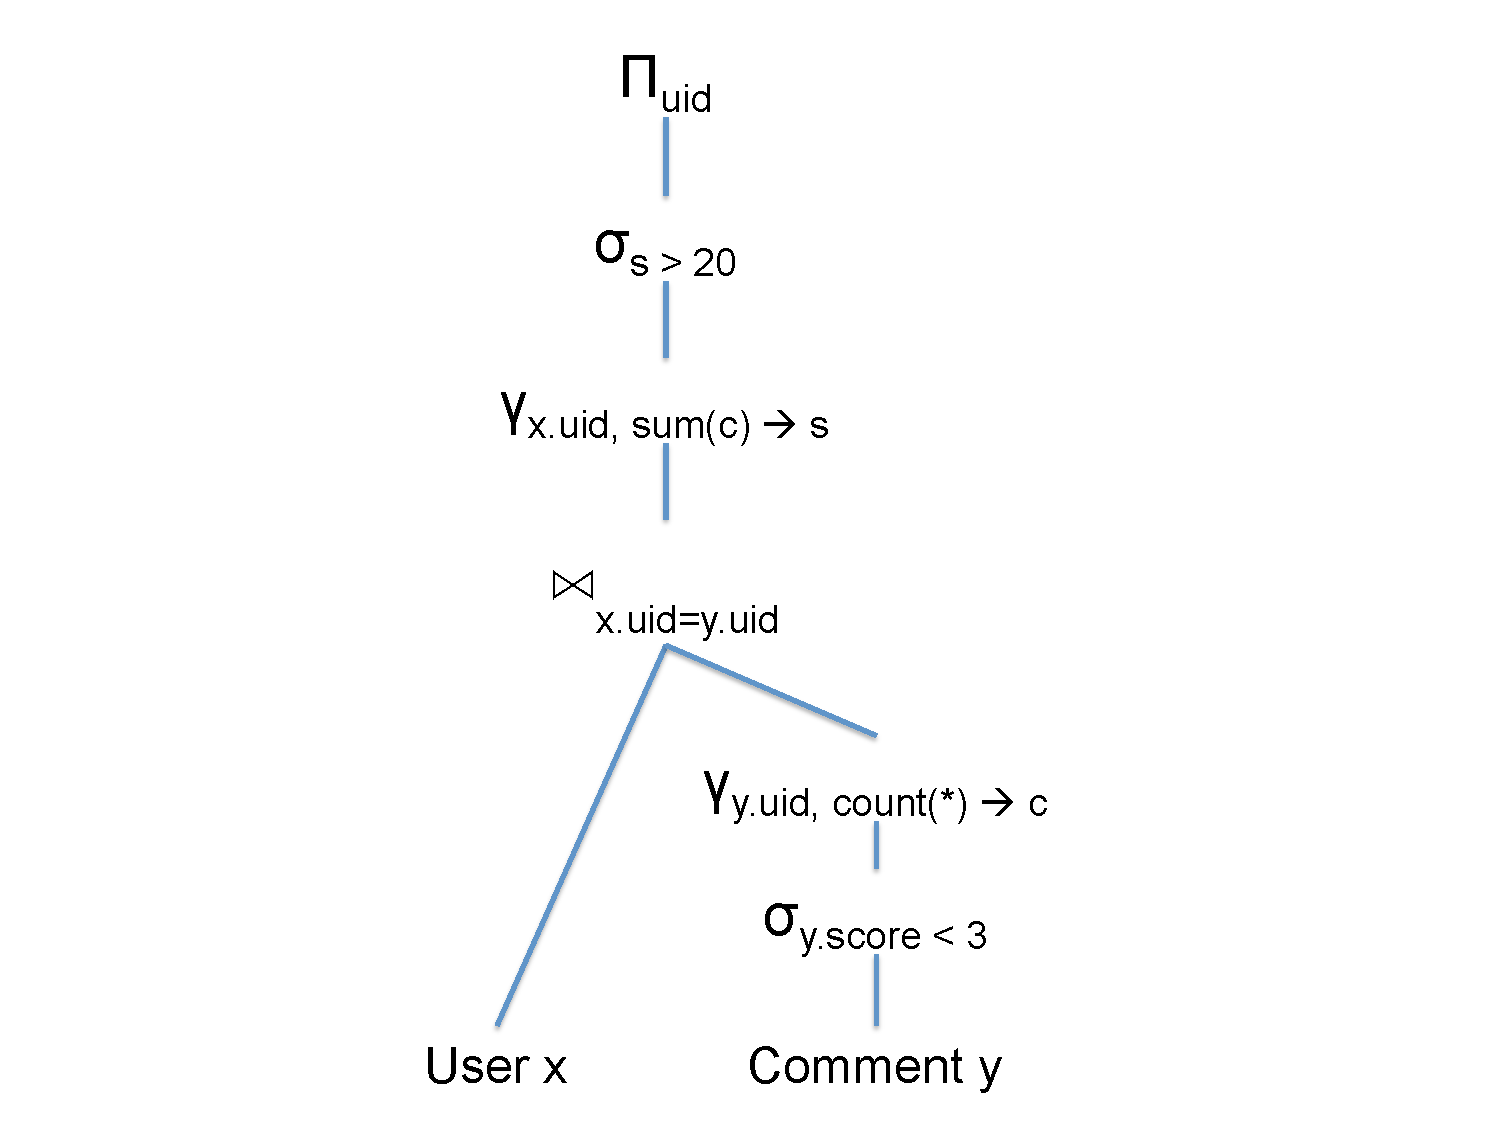
\includegraphics[scale=0.4]{FIGS/ra}

Write an equivalent SQL query {\em without} using any subqueries.

\begin{solution}
\begin{verbatim}
select x.uid
from Users x, Comment y
where x.uid = y.uid and y.score < 3
group by x.uid
having count(*) > 20
\end{verbatim}
\end{solution}

\newpage

{\scriptsize
\hfill
\begin{tabular}{l}
  \texttt{Users(\underline{uid}, name)} \\
  \texttt{Comment(uid, pid, score, txt)} \\
  \texttt{Picture(\underline{pid}, author, img)}
\end{tabular}
}

\part[10] Consider the following query in the relational calculus:

  \begin{align*}
    Q(u,n) = \texttt{Users}(u,n) \wedge \forall p.\forall  i.\left(\texttt{Picture}(p,u,i) \Rightarrow \forall v.\forall s.\forall  t.\left(\texttt{Comment}(v,p,s,t) \Rightarrow s > 5\right)\right)
  \end{align*}

Write an equivalent expression that does not use a universal
quantifier.

\begin{solution}
    \begin{align*}
    Q(u,n) = \texttt{Users}(u,n) \wedge \neg \exists p.\exists  i.\left(\texttt{Picture}(p,u,i) \wedge \exists v.\exists s.\exists  t.\left(\texttt{Comment}(v,p,s,t) \wedge s \leq 5\right)\right)
  \end{align*}
\end{solution}

\newpage

\end{parts}

\section{XML and XPath}


\question (\totalpoints\ \points) 


\begin{parts}
  \part[10] Consider the XML document below:

\begin{verbatim}
<a>
  <a>
    <a> 1 </a>
    <a> 2 </a>
  </a>
  <a>
    <a> 3 </a>
    <a> 4 </a>
  </a>
</a>
\end{verbatim}
 For each of the XPath queries below, indicate how many elements the
 expression returns:

\eat{
%%%% Run Saxon on the files q1.xq, ..., q5.xq to check the answers
}

 \begin{subparts}
   \subpart \verb+//a+ \answerline[7]{Answer}
   \subpart \verb+//a[a/text()=3]/a+ \answerline[2]{Answer}
   \subpart \verb+//a[a/a/text()=3]/a/a+ \answerline[4]{Answer}
   \subpart \verb+//a[a/text()=2][a/text()=3]+ \answerline[0]{Answer}
   \subpart \verb+//a[a/a/text()=2][a/a/text()=3]+ \answerline[1]{Answer}
 \end{subparts}

\newpage

\part[10] For each statement below indicate whether it is true of
false.

\begin{subparts}
  \subpart XML databases are replacing relational databases in today's
  enterprise applications.  \answerline[False]{True or false?}

  \subpart Compared to relational data, XML data is easier to exchange
  between applications or between users.  \answerline[True]{True or
    false?}

  \subpart The XPath expressions \verb+/a/b[@c='5'][@d='2']+ and
  \verb+/a/b[@d='2'][@c='5']+ are equivalent.  \answerline[True]{True
    or false?}

  \subpart The XPath expressions \verb+/a/b[@c='5'][2]+ and
  \verb+/a/b[2][@c='5']+ are equivalent. \answerline[False]{True or
    false?}

  \subpart The XPath expressions \verb+/a/*//b+ and \verb+/a//*/b+ are
  equivalent.  \answerline[True]{True or false?}
\end{subparts}


\end{parts}

\end{questions}
\end{document}
